%-----------------------------------------------------------------------
% Beginning of chap2.tex
%-----------------------------------------------------------------------
%
%  AMS-LaTeX sample file for a chapter of a monograph, to be used with
%  an AMS monograph document class.  This is a data file input by
%  chapter.tex.
%
%  Use this file as a model for a chapter; DO NOT START BY removing its
%  contents and filling in your own text.
% 
%%%%%%%%%%%%%%%%%%%%%%%%%%%%%%%%%%%%%%%%%%%%%%%%%%%%%%%%%%%%%%%%%%%%%%%%


\chapter*{Lecture 14}
\addcontentsline{toc}{chapter}{Lecture 14}
\addtocounter{chapter}{14}
%\addtocounter{section}{-2}
%\numberwithin{section}{chapter}
\numberwithin{equation}{chapter}
\numberwithin{theorem}{chapter}

%\epigraph{}{--- \textup{}}

So far we have only dealt with constrained optimization problems where the objective and the constraints are linear. We now turn attention to general problems of the form

\begin{align*}\label{eq:constr}\tag{1}
\begin{split}
 \minimize & f(\vct{x})\\
 \subjto & \vct{g}(\vct{x})\leq \zerovct\\
         & \vct{h}(\vct{x})= \zerovct,
\end{split}
\end{align*}
where $\vct{x}\in \R^n$, $\vct{g}=(g_1,\dots,g_m)^{\trans}$, $\vct{g}=(g_1,\dots,g_{\ell})$, and the inequalities are componentwise. 
The problem~\eqref{eq:constr} is {\em convex}, if $f$ and the $g_i$ are convex, and the $h_j$ are linear. We also denote by $\mathrm{dom}(f)$ the {\em domain} of $f$, which is the set of points $\vct{x}$ where $f$ takes a finite value. The feasible set
\begin{equation*}
 \mathcal{F} = \{\vct{x} \mid g_i(\vct{x})\leq 0, \ h_j(\vct{x})=0, \ 1\leq i\leq m, \ 1\leq j\leq \ell\}
\end{equation*}
for a convex constrained problem is a convex set.

\section{Quadratic Programming and Portfolio Optimization}


\begin{example} (Portfolio optimization)
If we invest an amount $x^0$ into a product at period $0$, and at period $1$ (for example, one day) the value is $x^1$, then the \textbf{relative return} is defined as
\begin{equation*}
  r = \frac{x^{1}-x^{0}}{x^{0}}.
\end{equation*}
As we can't predict the future, we usually work with the \textbf{expected return}, which is a statistical estimate of the future return. One naive method of estimating the future return is by taking the average of past returns, but other more sophisticated methods are possible.
In \textbf{portfolio optimization}, we have a proportion $x_i$ of our available funds that we want to invest in a stock $i$ with expected return $r_i$ (in particular, as $x_i$ measures a proportion, we have $\sum_{i=1}^n x_i = 1$). We may or may not allow $x_i<0$, which would correspond to short-selling or borrowing.  
 The total expected return is then $\vct{x}^{\trans}\vct{r}=\sum_{i=1}^n x_ir_i$. 
 
 The \textbf{risk} is an investment is measured in terms of the \textbf{covariance matrix} $\mtx{\Sigma}$. The $(i,j)$-th entry of the covariance matrix is the covariance between the returns of products $i$ and $j$, and is estimated using statistical methods. More precisely, the risk of the investment is measured by the quadratic function $\vct{x}^{\trans}\Sigma\vct{x}$, where $\vct{x}$ is the vector of positions in each asset. A portfolio optimization problem either seeks to maximize the return while bounding the risk,
 \begin{align*}
  \maximize & \vct{x}^{\trans}\vct{r}\\
  \subjto & \vct{x}^{\trans}\mtx{\Sigma}\vct{x}\leq \sigma,\\
  & \sum_{i=1}^n x_i=1\\
  & x_i\geq 0,
 \end{align*}
or minimize the risk given a certain target return $\mu$,
\begin{align*}
 \minimize & \vct{x}^{\trans}\mtx{\Sigma}\vct{x}\\
 \subjto & \vct{x}^{\trans}\vct{r} = \mu\\
 & \sum_{i=1}^n x_i = 1\\
 & x_i\geq 0.
\end{align*}
Both of these problems are convex optimization problems. The constraints $x_i\geq 0$ mean that we are not allowed to short-sell; when dealing with futures or options, or if we are a large institutional investor, we may drop these constraints.
\end{example}

\begin{remark}
 There are many problems of interest which are not convex, but in some cases it is possible to formulate an {\em equivalent} convex optimization problem. For example, consider the optimization problem
 \begin{equation}\label{eq:ex1}
  \minimize x_1^2+x_2^2 \quad \subjto \frac{x_1}{1+x_2^2}\leq 0, \ (x_1+x_2)^2=0.
 \end{equation}
This problem is not a convex optimization problem (why?). However, the following problem
\begin{equation}\label{eq:ex2}
 \minimize x_1^2+x_2^2 \quad \subjto x_1\leq 0, \ x_1+x_2=0
\end{equation}
is clearly convex, and the solution of~\eqref{eq:ex1} coincides with the solution of~\eqref{eq:ex2}.
\end{remark}

\section{First order optimality conditions}
So far we have seen two examples of first order optimality conditions: for unconstraint optimization ($\nabla f(\vct{x})=0$) and for linear programming. We now generalize these to the setting of constrained convex optimization.

\begin{theorem}
 Let $f\colon \R^d\to \R$ be a convex, differentiable function, and 
 \begin{equation*}
  \mathcal{F}=\{\vct{x} \mid g_i(\vct{x})\leq 0, \ h_j(\vct{x})=0, \ 1\leq i\leq m, \ 1\leq j\leq \ell\}
 \end{equation*}
a feasible set, with $g_i$ convex and $h_j$ linear. Then $\vct{x}^*$ is an optimal point of the optimization problem
\begin{equation*}
 \minimize f(\vct{x}) \ \subjto \vct{x}\in \mathcal{F}
\end{equation*}
if and only if for all $\vct{y}\in \mathcal{F}$, 
\begin{equation}\label{eq:opt}
 \ip{\nabla f(\vct{x}^*)}{\vct{y}-\vct{x}^*}\geq 0.
\end{equation}
\end{theorem}

\begin{proof}
 Suppose $\vct{x}^*$ is such that~\eqref{eq:constr} holds. Then, since $f$ is a convex function,
 for all $\vct{y}\in \mathcal{F}$ we have, by Theorem 2.4.1,
 \begin{equation*}
  f(\vct{y})\geq f(\vct{x}^*)+\ip{\nabla f(\vct{x}^*)}{\vct{y}-\vct{x}^*} \geq f(\vct{x}^*),
 \end{equation*}
which shows that $\vct{x}^*$ is a minimizer in $\mathcal{F}$. To show the opposite direction, assume that $\vct{x}^*$ is a minimizer but that~\eqref{eq:constr} does not hold. This means that there exists a $\vct{y}\in \mathcal{F}$ such that $\ip{\nabla f(\vct{x}^*)}{\vct{y}-\vct{x}^*}<0$. Since both $\vct{x}^*$ and $\vct{y}$ are in $\mathcal{F}$ and $\mathcal{F}$ is convex, any point $\vct{z}(\lambda)=(1-\lambda)\vct{x}^*+t\vct{y}$ with $\lambda\in [0,1]$ is also in $\mathcal{F}$. At $\lambda=0$ we have
\begin{equation*}
 \frac{df}{d\lambda}f(\vct{z}(\lambda))|_{\lambda=0} = \ip{\nabla f(\vct{x}^*)}{\vct{y}-\vct{x}^*}<0.
\end{equation*}
Since the derivative at $\lambda=0$ is negative, the function $f(\vct{z}(\lambda))$ is decreasing at $\lambda=0$, and therefore, for small $\lambda>0$, $f(\vct{z}(\lambda))<f(\vct{z}(0))=f(\vct{x}^*)$, in contradiction to the assumption that $\vct{x}^*$ is a minimizer.
\end{proof}

\begin{example}
 In the absence of constraints, $\mathcal{F}=\R^d$, and the statement says that
 \begin{equation*}
  \forall \vct{y}\in \R^d\colon \ip{\nabla f(\vct{x}^*)}{\vct{y}-\vct{x}^*}\geq 0.
 \end{equation*}
If there was a $\vct{y}$ such that $\ip{\nabla f(\vct{x}^*)}{\vct{y}-\vct{x}^*}>0$, then replacing $\vct{y}$ by $2\vct{x}-\vct{y}$ we also have the converse inequality, and therefore the optimality condition is equivalent to saying that $\nabla f(\vct{x}^*)=\zerovct$. We therefore recover the well-known first order optimality condition from Lecture 2. 
\end{example}

Geometrically, the first order optimality condition means that the set
\begin{equation*}
 \{\vct{x}\mid \ip{\nabla f(\vct{x}^*)}{\vct{x}}=\ip{\nabla f(\vct{x}^*)}{\vct{x}^*}\}
\end{equation*}
defines a supporting hyperplane to the set $\mathcal{F}$.

\begin{figure}[h!]
\centering
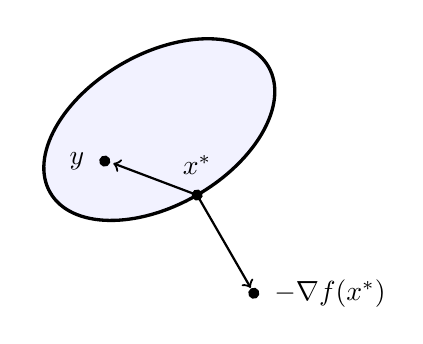
\begin{tikzpicture}[thick,rotate=30,scale=0.8]
\filldraw[color=black, fill=blue!5, very thick](0,0) ellipse (2 and 1.2);
\node (A1) at (0,-3)  [label=0:{$-\nabla f(\vct{x}^*)$}] {};
\node (A2) at (0,-1.2)  [label=90:{$\vct{x}^*$}] {};
%\node (A3) at (0,-2.5)  [label=180:{$\vct{a}$}] {};
\node (A4) at (-1,0)  [label=180:{$\vct{y}$}] {};
\filldraw[black] (0,-3) circle (2pt);
\filldraw[black] (0,-1.2) circle (2pt);
\filldraw[black] (-1,0) circle (2pt);
\draw[color=black, thick, <-] (0,-2.9) -- (0,-1.2);
\draw[color=black, thick, <-] (-0.9,-0.1) -- (0,-1.2);
\end{tikzpicture}
\caption{Optimality condition} \label{fig:neg}
\end{figure}

% %-----------------------------------------------------------------------
% % End of chap1.tex
% %-----------------------------------------------------------------------
